\subchapter{Podstawy programowania dynamicznego}

\exercise %15.3-1
Efektywniejszą metodą znajdowania optymalnego nawiasowania iloczynu ciągu macierzy jest wywołanie procedury \proc{Recursive-Matrix-Chain}.
Aby się o~tym przekonać, przyjrzyjmy się działaniu obu metod dla podciągu $A_iA_{i+1}\dots A_j$.

Procedura \proc{Recursive-Matrix-Chain} tworzy podziały tego podciągu na dwie części i~rekurencyjnie rozwiązuje powstałe podproblemy.
Dokładniej, dla każdego $k=i$, $i+1$, \dots, $j-1$ oddzielnie znajduje rozwiązanie dla podciągu $A_iA_{i+1}\dots A_k$ i~podciągu $A_{k+1}A_{k+2}\dots A_j$, a~następnie łączy te rozwiązania, aby otrzymać rozwiązanie dla $A_iA_{i+1}\dots A_j$.

Z~kolei w~trakcie generowania wszystkich poprawnych nawiasowań podciągu $A_iA_{i+1}\dots A_j$, dla każdego $k=i$, $i+1$, \dots, $j-1$ i~każdego poprawnego nawiasowania podciągu $A_iA_{i+1}\dots A_k$ zostanie rozważone każde poprawne nawiasowanie podciągu $A_{k+1}A_{k+2}\dots A_j$.
Oczywistym jest, że to podejście wymaga znacznie większej liczby operacji.
Jest tak dlatego, że nie wykorzystuje ono własności optymalnej podstruktury tego problemu.

\exercise %15.3-2
Sortowanie przez scalanie jest algorytmem realizującym podejście ,,dziel i~zwyciężaj'', w~którym początkowy problem dzielony jest na podproblemy rozwiązywane rekurencyjnie.
Powstające podproblemy nie powtarzają się pomiędzy wywołaniami rekurencyjnymi, co można zaobserwować na ilustracji drzewa rekursji tego algorytmu (rys.\ \ref{fig:15.3-2}).
W~drzewie tym każdy węzeł jest unikalny, inaczej niż w~przypadku drzewa rekursji algorytmu opartego na programowaniu dynamicznym, np.\ tego z~rys.\ 15.5 z Podręcznika.
Brak wspólnych podproblemów w~algorytmach opartych na metodzie ,,dziel i~zwyciężaj'' sprawia, że nie można ich przyspieszyć, stosując spamiętywanie.
\begin{figure}[!ht]
	\centering 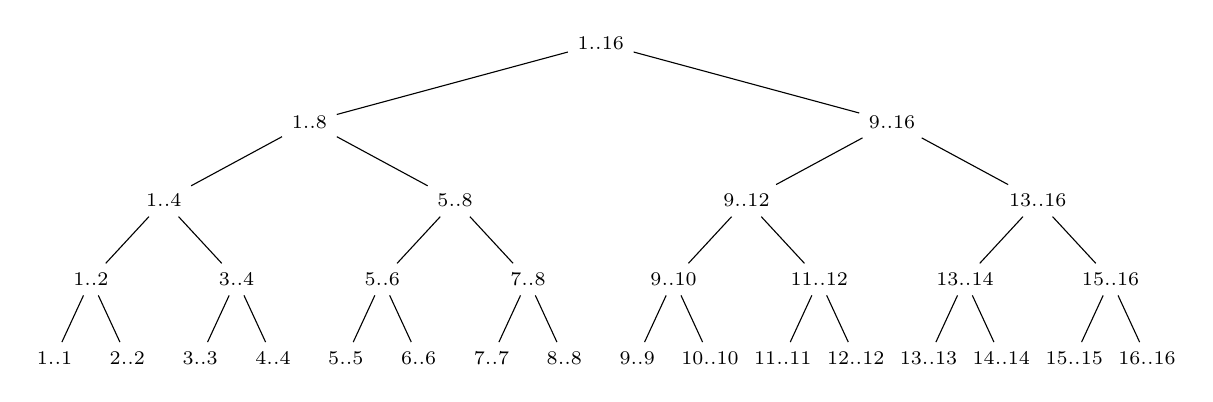
\begin{tikzpicture}[
	level/.append style = {level distance=10mm, sibling distance=148mm/2^#1},
	every node/.append style = {font=\scriptsize}
]

\node (root) {$1..16$}
	child {node {$1..8$}
		child {node {$1..4$}
			child {node {$1..2$}
				child {node {$1..1$}}
				child {node {$2..2$}}
			}
			child {node {$3..4$}
				child {node {$3..3$}}
				child {node {$4..4$}}
			}
		}
		child {node {$5..8$}
			child {node {$5..6$}
				child {node {$5..5$}}
				child {node {$6..6$}}
			}
			child {node {$7..8$}
				child {node {$7..7$}}
				child {node {$8..8$}}
			}
		}
	}
	child {node {$9..16$}
		child {node {$9..12$}
			child {node {$9..10$}
				child {node {$9..9$}}
				child {node {$10..10$}}
			}
			child {node {$11..12$}
				child {node {$11..11$}}
				child {node {$12..12$}}
			}
		}
		child {node {$13..16$}
			child {node {$13..14$}
				child {node {$13..13$}}
				child {node {$14..14$}}
			}
			child {node {$15..16$}
				child {node {$15..15$}}
				child {node {$16..16$}}
			}
		}
	};

\end{tikzpicture}

	\caption{Drzewo rekursji dla procedury \proc{Merge-Sort} działającej na tablicy z~16 elementami.
Każdy węzeł drzewa jest oznaczony zakresem $i\twodots j$ tablicy, na której działa procedura.} \label{fig:15.3-2}
\end{figure}

\exercise %15.3-3
Problem ten ma własność optymalnej podstruktury, o~czym można się przekonać podobnie, jak w~jego oryginalnej wersji.
W~tym wariancie optymalnym nawiasowaniem iloczynu macierzy będziemy nazywać takie nawiasowanie, które maksymalizuje liczbę mnożeń skalarnych.

Przypuśćmy, że w~optymalnym nawiasowaniu iloczynu $A_iA_{i+1}\dots A_j$ podział występuje między $A_k$ i~$A_{k+1}$.
Wówczas nawiasowanie podciągu $A_iA_{i+1}\dots A_k$, stanowiące część optymalnego nawiasowania iloczynu $A_iA_{i+1}\dots A_j$, musi być optymalne.
Gdyby bowiem istniał sposób ustawienia nawiasów w~ciągu $A_iA_{i+1}\dots A_k$ o~większym koszcie, to podmieniając nawiasowanie tego podciągu w~optymalnym nawiasowaniu $A_iA_{i+1}\dots A_j$, otrzymalibyśmy inne nawiasowanie dla $A_iA_{i+1}\dots A_j$, ale o~koszcie większym niż optymalny, co stanowi sprzeczność z~założeniem.
Podobne rozumowanie prowadzi do wniosku, że nawiasowanie podciągu $A_{k+1}A_{k+2}\dots A_j$ w~optymalnym nawiasowaniu $A_iA_{i+1}\dots A_j$ jest optymalne dla ciągu $A_{k+1}A_{k+2}\dots A_j$.

\exercise %15.3-4
W~problemie planowania czynności na liniach montażowych zarówno najszybszy sposób montażu do stanowiska $S_{1,j}$, jak i~najszybszy sposób montażu do stanowiska $S_{2,j}$, polega na optymalnych czasach montażu do stanowisk $S_{1,j-1}$ i~$S_{2,j-1}$.
Innymi słowy, wartości $f_1[j-1]$ oraz $f_2[j-1]$ wykorzystywane są do obliczenia zarówno $f_1[j]$, jak i~$f_2[j]$.

\exercise %15.3-5
Jednym z~kontrprzykładów jest ciąg macierzy $\langle A_1,A_2,A_3\rangle$ o~rozmiarach stanowiących ciąg $\langle1,2,5,4\rangle$.
Liczbą mnożeń skalarnych wykonywanych podczas mnożenia $A_1$ przez $(A_2A_3)$ jest $1\cdot2\cdot4=8$, a~podczas mnożenia $(A_1A_2)$ przez $A_3$ -- $1\cdot5\cdot4=20$.
W~podejściu zachłannym podział iloczynu $A_1A_2A_3$ zostanie zatem wyznaczony między macierzą $A_1$ a~$A_2$ i~wynikowym nawiasowaniem będzie $(A_1(A_2A_3))$ z~kosztem $2\cdot5\cdot4+1\cdot2\cdot4=48$ mnożeń skalarnych.
Rozwiązaniem optymalnym jest jednak nawiasowanie $((A_1A_2)A_3)$ o~koszcie $1\cdot2\cdot5+1\cdot5\cdot4=30$.
